% Options for packages loaded elsewhere
\PassOptionsToPackage{unicode}{hyperref}
\PassOptionsToPackage{hyphens}{url}
%
\documentclass[
]{article}
\usepackage{lmodern}
\usepackage{amssymb,amsmath}
\usepackage{ifxetex,ifluatex}
\ifnum 0\ifxetex 1\fi\ifluatex 1\fi=0 % if pdftex
  \usepackage[T1]{fontenc}
  \usepackage[utf8]{inputenc}
  \usepackage{textcomp} % provide euro and other symbols
\else % if luatex or xetex
  \usepackage{unicode-math}
  \defaultfontfeatures{Scale=MatchLowercase}
  \defaultfontfeatures[\rmfamily]{Ligatures=TeX,Scale=1}
\fi
% Use upquote if available, for straight quotes in verbatim environments
\IfFileExists{upquote.sty}{\usepackage{upquote}}{}
\IfFileExists{microtype.sty}{% use microtype if available
  \usepackage[]{microtype}
  \UseMicrotypeSet[protrusion]{basicmath} % disable protrusion for tt fonts
}{}
\makeatletter
\@ifundefined{KOMAClassName}{% if non-KOMA class
  \IfFileExists{parskip.sty}{%
    \usepackage{parskip}
  }{% else
    \setlength{\parindent}{0pt}
    \setlength{\parskip}{6pt plus 2pt minus 1pt}}
}{% if KOMA class
  \KOMAoptions{parskip=half}}
\makeatother
\usepackage{xcolor}
\IfFileExists{xurl.sty}{\usepackage{xurl}}{} % add URL line breaks if available
\IfFileExists{bookmark.sty}{\usepackage{bookmark}}{\usepackage{hyperref}}
\hypersetup{
  hidelinks,
  pdfcreator={LaTeX via pandoc}}
\urlstyle{same} % disable monospaced font for URLs
\usepackage[margin=1in]{geometry}
\usepackage{color}
\usepackage{fancyvrb}
\newcommand{\VerbBar}{|}
\newcommand{\VERB}{\Verb[commandchars=\\\{\}]}
\DefineVerbatimEnvironment{Highlighting}{Verbatim}{commandchars=\\\{\}}
% Add ',fontsize=\small' for more characters per line
\usepackage{framed}
\definecolor{shadecolor}{RGB}{248,248,248}
\newenvironment{Shaded}{\begin{snugshade}}{\end{snugshade}}
\newcommand{\AlertTok}[1]{\textcolor[rgb]{0.94,0.16,0.16}{#1}}
\newcommand{\AnnotationTok}[1]{\textcolor[rgb]{0.56,0.35,0.01}{\textbf{\textit{#1}}}}
\newcommand{\AttributeTok}[1]{\textcolor[rgb]{0.77,0.63,0.00}{#1}}
\newcommand{\BaseNTok}[1]{\textcolor[rgb]{0.00,0.00,0.81}{#1}}
\newcommand{\BuiltInTok}[1]{#1}
\newcommand{\CharTok}[1]{\textcolor[rgb]{0.31,0.60,0.02}{#1}}
\newcommand{\CommentTok}[1]{\textcolor[rgb]{0.56,0.35,0.01}{\textit{#1}}}
\newcommand{\CommentVarTok}[1]{\textcolor[rgb]{0.56,0.35,0.01}{\textbf{\textit{#1}}}}
\newcommand{\ConstantTok}[1]{\textcolor[rgb]{0.00,0.00,0.00}{#1}}
\newcommand{\ControlFlowTok}[1]{\textcolor[rgb]{0.13,0.29,0.53}{\textbf{#1}}}
\newcommand{\DataTypeTok}[1]{\textcolor[rgb]{0.13,0.29,0.53}{#1}}
\newcommand{\DecValTok}[1]{\textcolor[rgb]{0.00,0.00,0.81}{#1}}
\newcommand{\DocumentationTok}[1]{\textcolor[rgb]{0.56,0.35,0.01}{\textbf{\textit{#1}}}}
\newcommand{\ErrorTok}[1]{\textcolor[rgb]{0.64,0.00,0.00}{\textbf{#1}}}
\newcommand{\ExtensionTok}[1]{#1}
\newcommand{\FloatTok}[1]{\textcolor[rgb]{0.00,0.00,0.81}{#1}}
\newcommand{\FunctionTok}[1]{\textcolor[rgb]{0.00,0.00,0.00}{#1}}
\newcommand{\ImportTok}[1]{#1}
\newcommand{\InformationTok}[1]{\textcolor[rgb]{0.56,0.35,0.01}{\textbf{\textit{#1}}}}
\newcommand{\KeywordTok}[1]{\textcolor[rgb]{0.13,0.29,0.53}{\textbf{#1}}}
\newcommand{\NormalTok}[1]{#1}
\newcommand{\OperatorTok}[1]{\textcolor[rgb]{0.81,0.36,0.00}{\textbf{#1}}}
\newcommand{\OtherTok}[1]{\textcolor[rgb]{0.56,0.35,0.01}{#1}}
\newcommand{\PreprocessorTok}[1]{\textcolor[rgb]{0.56,0.35,0.01}{\textit{#1}}}
\newcommand{\RegionMarkerTok}[1]{#1}
\newcommand{\SpecialCharTok}[1]{\textcolor[rgb]{0.00,0.00,0.00}{#1}}
\newcommand{\SpecialStringTok}[1]{\textcolor[rgb]{0.31,0.60,0.02}{#1}}
\newcommand{\StringTok}[1]{\textcolor[rgb]{0.31,0.60,0.02}{#1}}
\newcommand{\VariableTok}[1]{\textcolor[rgb]{0.00,0.00,0.00}{#1}}
\newcommand{\VerbatimStringTok}[1]{\textcolor[rgb]{0.31,0.60,0.02}{#1}}
\newcommand{\WarningTok}[1]{\textcolor[rgb]{0.56,0.35,0.01}{\textbf{\textit{#1}}}}
\usepackage{graphicx,grffile}
\makeatletter
\def\maxwidth{\ifdim\Gin@nat@width>\linewidth\linewidth\else\Gin@nat@width\fi}
\def\maxheight{\ifdim\Gin@nat@height>\textheight\textheight\else\Gin@nat@height\fi}
\makeatother
% Scale images if necessary, so that they will not overflow the page
% margins by default, and it is still possible to overwrite the defaults
% using explicit options in \includegraphics[width, height, ...]{}
\setkeys{Gin}{width=\maxwidth,height=\maxheight,keepaspectratio}
% Set default figure placement to htbp
\makeatletter
\def\fps@figure{htbp}
\makeatother
\setlength{\emergencystretch}{3em} % prevent overfull lines
\providecommand{\tightlist}{%
  \setlength{\itemsep}{0pt}\setlength{\parskip}{0pt}}
\setcounter{secnumdepth}{-\maxdimen} % remove section numbering

\author{}
\date{\vspace{-2.5em}}

\begin{document}

\hypertarget{chap-stan}{%
\section{Stan for Bayesian time series analysis}\label{chap-stan}}

\chaptermark{Stan}

For this lab, we will use \href{http://mc-stan.org/documentation/}{Stan}
for fitting models. These examples are primarily drawn from the Stan
manual and previous code from this class.

A script with all the R code in the chapter can be downloaded
\href{./Rcode/fitting-models-with-stan.R}{here}.

\hypertarget{data-and-packages}{%
\subsubsection*{Data and packages}\label{data-and-packages}}
\addcontentsline{toc}{subsubsection}{Data and packages}

You will need the \textbf{atsar} package we have written for fitting
state-space time series models with Stan. This is hosted on Github
\href{https://github.com/nwfsc-timeseries/atsar}{safs-timeseries}.
Install using the \textbf{devtools} package.

\begin{Shaded}
\begin{Highlighting}[]
\KeywordTok{library}\NormalTok{(devtools)}
\CommentTok{# Windows users will likely need to set this}
\CommentTok{# Sys.setenv('R_REMOTES_NO_ERRORS_FROM_WARNINGS' = 'true')}
\NormalTok{devtools}\OperatorTok{::}\KeywordTok{install_github}\NormalTok{(}\StringTok{"nwfsc-timeseries/atsar"}\NormalTok{)}
\NormalTok{devtools}\OperatorTok{::}\KeywordTok{install_github}\NormalTok{(}\StringTok{"nwfsc-timeseries/tvvarss"}\NormalTok{)}
\NormalTok{devtools}\OperatorTok{::}\KeywordTok{install_github}\NormalTok{(}\StringTok{"fate-ewi/bayesdfa"}\NormalTok{)}
\end{Highlighting}
\end{Shaded}

In addition, you will need the \textbf{rstan}, \textbf{datasets},
\textbf{parallel} and \textbf{loo} packages. After installing, if
needed, load the packages:

\begin{Shaded}
\begin{Highlighting}[]
\KeywordTok{library}\NormalTok{(atsar)}
\KeywordTok{library}\NormalTok{(rstan)}
\KeywordTok{library}\NormalTok{(loo)}
\end{Highlighting}
\end{Shaded}

Once you have Stan and \textbf{rstan} installed, optimize Stan on your
machine:

\begin{Shaded}
\begin{Highlighting}[]
\KeywordTok{rstan_options}\NormalTok{(}\DataTypeTok{auto_write =} \OtherTok{TRUE}\NormalTok{)}
\KeywordTok{options}\NormalTok{(}\DataTypeTok{mc.cores =}\NormalTok{ parallel}\OperatorTok{::}\KeywordTok{detectCores}\NormalTok{())}
\end{Highlighting}
\end{Shaded}

For this lab, we will use a data set on airquality in New York from the
\textbf{datasets} package. Load the data and create a couple new
variables for future use.

\begin{Shaded}
\begin{Highlighting}[]
\KeywordTok{data}\NormalTok{(airquality, }\DataTypeTok{package =} \StringTok{"datasets"}\NormalTok{)}
\NormalTok{Wind <-}\StringTok{ }\NormalTok{airquality}\OperatorTok{$}\NormalTok{Wind  }\CommentTok{# wind speed}
\NormalTok{Temp <-}\StringTok{ }\NormalTok{airquality}\OperatorTok{$}\NormalTok{Temp  }\CommentTok{# air temperature}
\end{Highlighting}
\end{Shaded}

\hypertarget{sec-stan-lr}{%
\subsection{Linear regression}\label{sec-stan-lr}}

We'll start with the simplest time series model possible: linear
regression with only an intercept, so that the predicted values of all
observations are the same. There are several ways we can write this
equation. First, the predicted values can be written as
\(E[Y_{t}] = \beta x\), where \(x=1\). Assuming that the residuals are
normally distributed, the model linking our predictions to observed data
is written as \[y_t = \beta x + e_{t}, e_{t} \sim N(0,\sigma), x=1\]

An equivalent way to think about this model is that instead of the
residuals as normally distributed with mean zero, we can think of the
data \(y_t\) as being drawn from a normal distribution with a mean of
the intercept, and the same residual standard deviation:
\[Y_t \sim N(E[Y_{t}],\sigma)\] Remember that in linear regression
models, the residual error is interpreted as independent and identically
distributed observation error.

To run this model using our package, we'll need to specify the response
and predictor variables. The covariate matrix with an intercept only is
a matrix of 1s. To double check, you could always look at

\begin{Shaded}
\begin{Highlighting}[]
\NormalTok{x <-}\StringTok{ }\KeywordTok{model.matrix}\NormalTok{(}\KeywordTok{lm}\NormalTok{(Temp }\OperatorTok{~}\StringTok{ }\DecValTok{1}\NormalTok{))}
\end{Highlighting}
\end{Shaded}

Fitting the model using our function is done with this code,

\begin{Shaded}
\begin{Highlighting}[]
\NormalTok{lm_intercept <-}\StringTok{ }\NormalTok{atsar}\OperatorTok{::}\KeywordTok{fit_stan}\NormalTok{(}\DataTypeTok{y =} \KeywordTok{as.numeric}\NormalTok{(Temp), }\DataTypeTok{x =} \KeywordTok{rep}\NormalTok{(}\DecValTok{1}\NormalTok{, }
    \KeywordTok{length}\NormalTok{(Temp)), }\DataTypeTok{model_name =} \StringTok{"regression"}\NormalTok{)}
\end{Highlighting}
\end{Shaded}

Coarse summaries of \texttt{stanfit} objects can be examined by typing
one of the following

\begin{Shaded}
\begin{Highlighting}[]
\NormalTok{lm_intercept}
\CommentTok{# this is huge}
\KeywordTok{summary}\NormalTok{(lm_intercept)}
\end{Highlighting}
\end{Shaded}

But to get more detailed output for each parameter, you have to use the
\texttt{extract()} function,

\begin{Shaded}
\begin{Highlighting}[]
\NormalTok{pars <-}\StringTok{ }\NormalTok{rstan}\OperatorTok{::}\KeywordTok{extract}\NormalTok{(lm_intercept)}
\KeywordTok{names}\NormalTok{(pars)}
\end{Highlighting}
\end{Shaded}

\begin{verbatim}
[1] "beta"    "sigma"   "pred"    "log_lik" "lp__"   
\end{verbatim}

\texttt{extract()} will return the draws from the posterior for your
parameters and any derived variables specified in your stan code. In
this case, our model is
\[y_t = \beta \times 1 + e_t, e_t \sim N(0,\sigma)\] so our estimated
parameters are \(\beta\) and \(\sigma\). Our stan code computed the
derived variables: predicted \(y_t\) which is
\(\hat{y}_t = \beta \times 1\) and the log-likelihood. lp\_\_ is the log
posterior which is automatically returned.

We can then make basic plots or summaries of each of these parameters,

\begin{Shaded}
\begin{Highlighting}[]
\KeywordTok{hist}\NormalTok{(pars}\OperatorTok{$}\NormalTok{beta, }\DecValTok{40}\NormalTok{, }\DataTypeTok{col =} \StringTok{"grey"}\NormalTok{, }\DataTypeTok{xlab =} \StringTok{"Intercept"}\NormalTok{, }\DataTypeTok{main =} \StringTok{""}\NormalTok{)}
\end{Highlighting}
\end{Shaded}

\begin{center}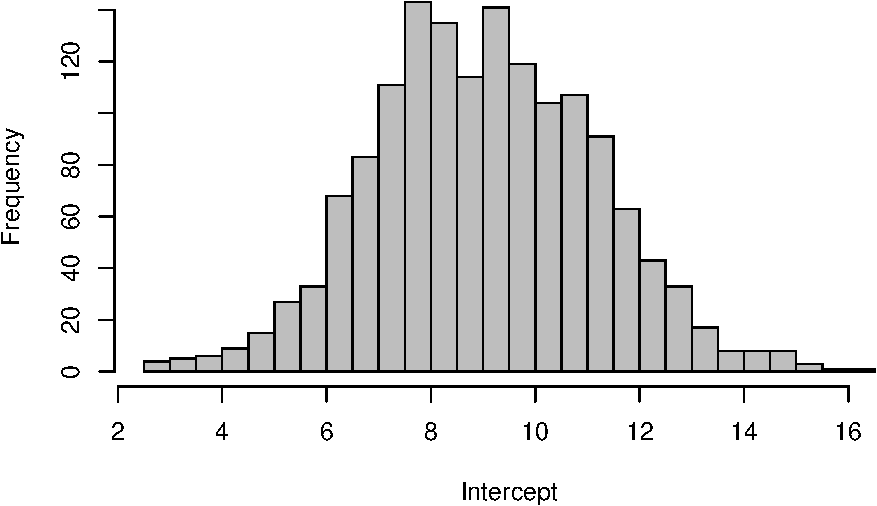
\includegraphics[width=0.8\linewidth]{fitting-models-with-stan_files/figure-latex/stan-hist-1} \end{center}

\begin{Shaded}
\begin{Highlighting}[]
\KeywordTok{quantile}\NormalTok{(pars}\OperatorTok{$}\NormalTok{beta, }\KeywordTok{c}\NormalTok{(}\FloatTok{0.025}\NormalTok{, }\FloatTok{0.5}\NormalTok{, }\FloatTok{0.975}\NormalTok{))}
\end{Highlighting}
\end{Shaded}

\begin{verbatim}
     2.5%       50%     97.5% 
 4.971048  8.980716 13.240347 
\end{verbatim}

One of the other useful things we can do is look at the predicted values
of our model (\(\hat{y}_t=\beta \times 1\)) and overlay the data. The
predicted values are \emph{pars\$pred}.

\begin{Shaded}
\begin{Highlighting}[]
\KeywordTok{plot}\NormalTok{(}\KeywordTok{apply}\NormalTok{(pars}\OperatorTok{$}\NormalTok{pred, }\DecValTok{2}\NormalTok{, mean), }\DataTypeTok{main =} \StringTok{"Predicted values"}\NormalTok{, }\DataTypeTok{lwd =} \DecValTok{2}\NormalTok{, }
    \DataTypeTok{ylab =} \StringTok{"Wind"}\NormalTok{, }\DataTypeTok{ylim =} \KeywordTok{c}\NormalTok{(}\KeywordTok{min}\NormalTok{(pars}\OperatorTok{$}\NormalTok{pred), }\KeywordTok{max}\NormalTok{(pars}\OperatorTok{$}\NormalTok{pred)), }
    \DataTypeTok{type =} \StringTok{"l"}\NormalTok{)}
\KeywordTok{lines}\NormalTok{(}\KeywordTok{apply}\NormalTok{(pars}\OperatorTok{$}\NormalTok{pred, }\DecValTok{2}\NormalTok{, quantile, }\FloatTok{0.025}\NormalTok{))}
\KeywordTok{lines}\NormalTok{(}\KeywordTok{apply}\NormalTok{(pars}\OperatorTok{$}\NormalTok{pred, }\DecValTok{2}\NormalTok{, quantile, }\FloatTok{0.975}\NormalTok{))}
\KeywordTok{points}\NormalTok{(Wind, }\DataTypeTok{col =} \StringTok{"red"}\NormalTok{)}
\end{Highlighting}
\end{Shaded}

\begin{figure}

{\centering 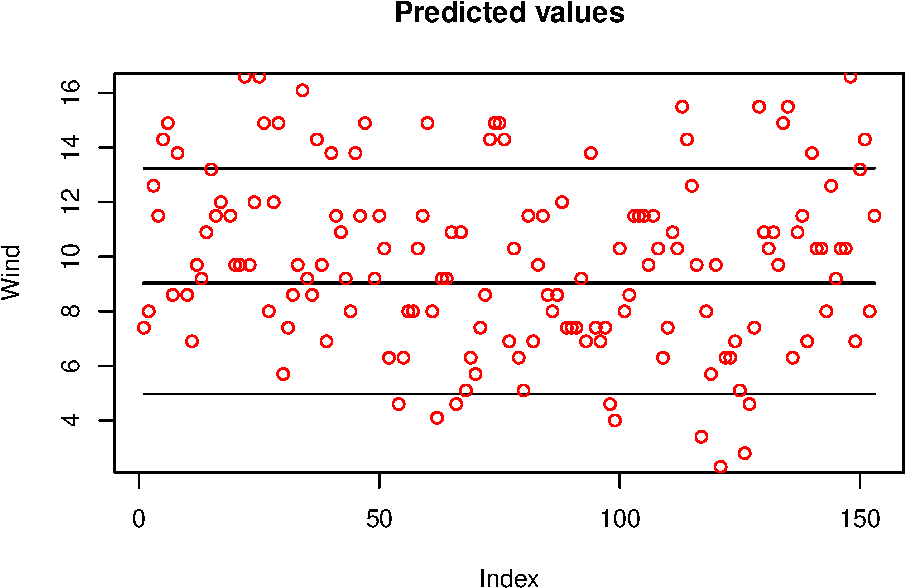
\includegraphics[width=0.8\linewidth]{fitting-models-with-stan_files/figure-latex/stan-fig-lm-1} 

}

\caption{Data and predicted values for the linear regression model.}\label{fig:stan-fig-lm}
\end{figure}

\hypertarget{sec-stan-burn}{%
\subsubsection{Burn-in and thinning}\label{sec-stan-burn}}

To illustrate the effects of the burn-in/warmup period and thinning, we
can re-run the above model, but for just 1 MCMC chain (the default is
3).

\begin{Shaded}
\begin{Highlighting}[]
\NormalTok{lm_intercept <-}\StringTok{ }\NormalTok{atsar}\OperatorTok{::}\KeywordTok{fit_stan}\NormalTok{(}\DataTypeTok{y =}\NormalTok{ Temp, }\DataTypeTok{x =} \KeywordTok{rep}\NormalTok{(}\DecValTok{1}\NormalTok{, }\KeywordTok{length}\NormalTok{(Temp)), }
    \DataTypeTok{model_name =} \StringTok{"regression"}\NormalTok{, }\DataTypeTok{mcmc_list =} \KeywordTok{list}\NormalTok{(}\DataTypeTok{n_mcmc =} \DecValTok{1000}\NormalTok{, }
        \DataTypeTok{n_burn =} \DecValTok{1}\NormalTok{, }\DataTypeTok{n_chain =} \DecValTok{1}\NormalTok{, }\DataTypeTok{n_thin =} \DecValTok{1}\NormalTok{))}
\end{Highlighting}
\end{Shaded}

\begin{verbatim}
Warning: There were 999 divergent transitions after warmup. See
http://mc-stan.org/misc/warnings.html#divergent-transitions-after-warmup
to find out why this is a problem and how to eliminate them.
\end{verbatim}

\begin{verbatim}
Warning: Examine the pairs() plot to diagnose sampling problems
\end{verbatim}

Here is a plot of the time series of \texttt{beta} with one chain and no
burn-in. Based on visual inspection, when does the chain converge?

\begin{Shaded}
\begin{Highlighting}[]
\NormalTok{pars <-}\StringTok{ }\NormalTok{rstan}\OperatorTok{::}\KeywordTok{extract}\NormalTok{(lm_intercept)}
\KeywordTok{plot}\NormalTok{(pars}\OperatorTok{$}\NormalTok{beta)}
\end{Highlighting}
\end{Shaded}

\begin{figure}

{\centering 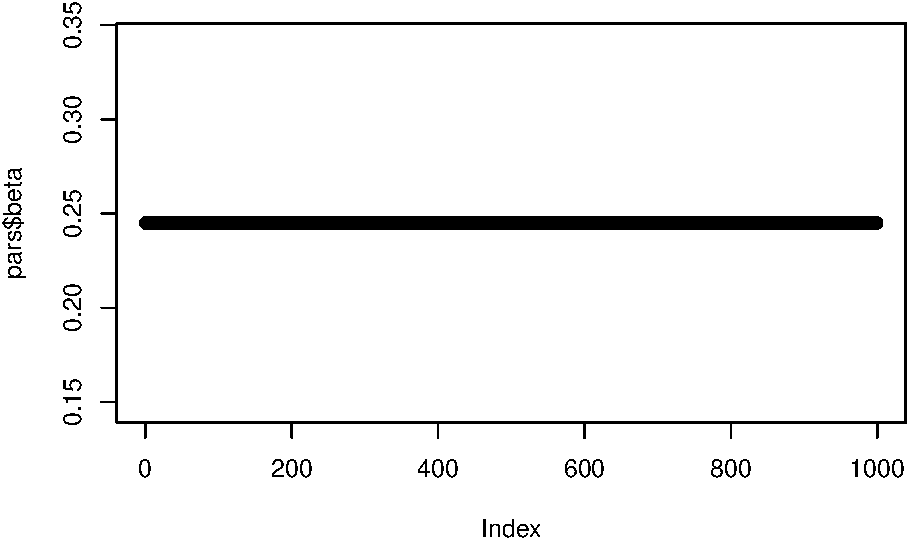
\includegraphics[width=0.8\linewidth]{fitting-models-with-stan_files/figure-latex/stan-fig-burnin-1} 

}

\caption{A time series of our posterior draws using one chain and no burn-in.}\label{fig:stan-fig-burnin}
\end{figure}

\hypertarget{sec-stan-lr-ar}{%
\subsection{Linear regression with correlated
errors}\label{sec-stan-lr-ar}}

In our first model, the errors were independent in time. We're going to
modify this to model autocorrelated errors. Autocorrelated errors are
widely used in ecology and other fields -- for a greater discussion, see
Morris and Doak (2002) Quantitative Conservation Biology. To make the
errors autocorrelated, we start by defining the error in the first time
step, \({e}_{1} = y_{1} - \beta\). The expectation of \({Y_t}\) in each
time step is then written as \[E[{Y_t}] = \beta + \phi  e_{t-1}\]

In addition to affecting the expectation, the correlation parameter
\(\phi\) also affects the variance of the errors, so that
\[{ \sigma  }^{ 2 }={ \psi  }^{ 2 }\left( 1-{ \phi  }^{ 2 } \right)\]
Like in our first model, we assume that the data follows a normal
likelihood (or equivalently that the residuals are normally
distributed), \(y_t = E[Y_t] + e_t\), or
\(Y_t \sim N(E[{Y_t}], \sigma)\). Thus, it is possible to express the
subsequent deviations as \({e}_{t} = {y}_{t} - E[{Y_t}]\), or
equivalently as \({e}_{t} = {y}_{t} - \beta -\phi {e}_{t-1}\).

We can fit this regression with autocorrelated errors by changing the
model name to `regression\_cor'

\begin{Shaded}
\begin{Highlighting}[]
\NormalTok{lm_intercept_cor <-}\StringTok{ }\NormalTok{atsar}\OperatorTok{::}\KeywordTok{fit_stan}\NormalTok{(}\DataTypeTok{y =}\NormalTok{ Temp, }\DataTypeTok{x =} \KeywordTok{rep}\NormalTok{(}\DecValTok{1}\NormalTok{, }\KeywordTok{length}\NormalTok{(Temp)), }
    \DataTypeTok{model_name =} \StringTok{"regression_cor"}\NormalTok{, }\DataTypeTok{mcmc_list =} \KeywordTok{list}\NormalTok{(}\DataTypeTok{n_mcmc =} \DecValTok{1000}\NormalTok{, }
        \DataTypeTok{n_burn =} \DecValTok{1}\NormalTok{, }\DataTypeTok{n_chain =} \DecValTok{1}\NormalTok{, }\DataTypeTok{n_thin =} \DecValTok{1}\NormalTok{))}
\end{Highlighting}
\end{Shaded}

\hypertarget{sec-stan-rw}{%
\subsection{Random walk model}\label{sec-stan-rw}}

All of the previous three models can be interpreted as observation error
models. Switching gears, we can alternatively model error in the state
of nature, creating process error models. A simple process error model
that many of you may have seen before is the random walk model. In this
model, the assumption is that the true state of nature (or latent
states) are measured perfectly. Thus, all uncertainty is originating
from process variation (for ecological problems, this is often
interpreted as environmental variation). For this simple model, we'll
assume that our process of interest (in this case, daily wind speed)
exhibits no daily trend, but behaves as a random walk.

\[y_t = y_{t-1} + e_{t}\]

And the \({e}_{t} \sim N(0, \sigma)\). Remember back to the
autocorrelated model (or MA(1) models) that we assumed that the errors
\(e_t\) followed a random walk. In contrast, this model assumes that the
errors are independent, but that the state of nature follows a random
walk. Note also that this model as written doesn't include a drift term
(this can be turned on / off using the \texttt{est\_drift} argument).

We can fit the random walk model using argument
\texttt{model\_name\ =\ \textquotesingle{}rw\textquotesingle{}} passed
to the \texttt{fit\_stan()} function.

\begin{Shaded}
\begin{Highlighting}[]
\NormalTok{rw <-}\StringTok{ }\NormalTok{atsar}\OperatorTok{::}\KeywordTok{fit_stan}\NormalTok{(}\DataTypeTok{y =}\NormalTok{ Temp, }\DataTypeTok{est_drift =} \OtherTok{FALSE}\NormalTok{, }\DataTypeTok{model_name =} \StringTok{"rw"}\NormalTok{)}
\end{Highlighting}
\end{Shaded}

\hypertarget{sec-stan-ar1}{%
\subsection{Autoregressive models}\label{sec-stan-ar1}}

A variation of the random walk model described previously is the
autoregressive time series model of order 1, AR(1). This model is
essentially the same as the random walk model but it introduces an
estimated coefficient, which we will call \(\phi\). The parameter
\(\phi\) controls the degree to which the random walk reverts to the
mean -- when \(\phi\) = 1, the model is identical to the random walk,
but at smaller values, the model will revert back to the mean (which in
this case is zero). Also, \(\phi\) can take on negative values, which
we'll discuss more in future lectures. The math to describe the AR(1)
model is: \[y_t = \phi y_{t-1} + e_{t}\].

The \texttt{fit\_stan()} function can fit higher order AR models, but
for now we just want to fit an AR(1) model and make a histogram of phi.

\begin{Shaded}
\begin{Highlighting}[]
\NormalTok{ar1 <-}\StringTok{ }\NormalTok{atsar}\OperatorTok{::}\KeywordTok{fit_stan}\NormalTok{(}\DataTypeTok{y =}\NormalTok{ Temp, }\DataTypeTok{x =} \KeywordTok{matrix}\NormalTok{(}\DecValTok{1}\NormalTok{, }\DataTypeTok{nrow =} \KeywordTok{length}\NormalTok{(Temp), }
    \DataTypeTok{ncol =} \DecValTok{1}\NormalTok{), }\DataTypeTok{model_name =} \StringTok{"ar"}\NormalTok{, }\DataTypeTok{est_drift =} \OtherTok{FALSE}\NormalTok{, }\DataTypeTok{P =} \DecValTok{1}\NormalTok{)}
\end{Highlighting}
\end{Shaded}

\hypertarget{sec-stan-uss}{%
\subsection{Univariate state-space models}\label{sec-stan-uss}}

At this point, we've fit models with observation or process error, but
we haven't tried to estimate both simultaneously. We will do so here,
and introduce some new notation to describe the process model and
observation model. We use the notation \({x_t}\) to denote the latent
state or state of nature (which is unobserved) at time \(t\) and
\({y_t}\) to denote the observed data. For introductory purposes, we'll
make the process model autoregressive (similar to our AR(1) model),

\[x_{t} = \phi  x_{t-1} + e_{t}, e_{t} \sim N(0,q)\]

For the process model, there are a number of ways to parameterize the
first `state', and we'll talk about this more in the class, but for the
sake of this model, we'll place a vague weakly informative prior on
\(x_1\), \(x_1 \sim N(0, 0.01)\).Second, we need to construct an
observation model linking the estimate unseen states of nature \(x_t\)
to the data \(y_t\). For simplicitly, we'll assume that the observation
errors are indepdendent and identically distributed, with no observation
component. Mathematically, this model is \[Y_t \sim N(x_t, r)\] In the
two above models, we'll refer to \(q\) as the standard deviation of the
process variance and \(r\) as the standard deviation of the observation
error variance

We can fit the state-space AR(1) and random walk models using the
\texttt{fit\_stan()} function:

\begin{Shaded}
\begin{Highlighting}[]
\NormalTok{ss_ar <-}\StringTok{ }\NormalTok{atsar}\OperatorTok{::}\KeywordTok{fit_stan}\NormalTok{(}\DataTypeTok{y =}\NormalTok{ Temp, }\DataTypeTok{est_drift =} \OtherTok{FALSE}\NormalTok{, }\DataTypeTok{model_name =} \StringTok{"ss_ar"}\NormalTok{)}
\NormalTok{ss_rw <-}\StringTok{ }\NormalTok{atsar}\OperatorTok{::}\KeywordTok{fit_stan}\NormalTok{(}\DataTypeTok{y =}\NormalTok{ Temp, }\DataTypeTok{est_drift =} \OtherTok{FALSE}\NormalTok{, }\DataTypeTok{model_name =} \StringTok{"ss_rw"}\NormalTok{)}
\end{Highlighting}
\end{Shaded}

\hypertarget{sec-stan-dfa}{%
\subsection{Dynamic factor analysis}\label{sec-stan-dfa}}

First load the plankton dataset from the \textbf{MARSS} package.

\begin{Shaded}
\begin{Highlighting}[]
\KeywordTok{library}\NormalTok{(MARSS)}
\KeywordTok{data}\NormalTok{(lakeWAplankton, }\DataTypeTok{package =} \StringTok{"MARSS"}\NormalTok{)}
\CommentTok{# we want lakeWAplanktonTrans, which has been transformed so}
\CommentTok{# the 0s are replaced with NAs and the data z-scored}
\NormalTok{dat <-}\StringTok{ }\NormalTok{lakeWAplanktonTrans}
\CommentTok{# use only the 10 years from 1980-1989}
\NormalTok{plankdat <-}\StringTok{ }\NormalTok{dat[dat[, }\StringTok{"Year"}\NormalTok{] }\OperatorTok{>=}\StringTok{ }\DecValTok{1980} \OperatorTok{&}\StringTok{ }\NormalTok{dat[, }\StringTok{"Year"}\NormalTok{] }\OperatorTok{<}\StringTok{ }\DecValTok{1990}\NormalTok{, }
\NormalTok{    ]}
\CommentTok{# create vector of phytoplankton group names}
\NormalTok{phytoplankton <-}\StringTok{ }\KeywordTok{c}\NormalTok{(}\StringTok{"Cryptomonas"}\NormalTok{, }\StringTok{"Diatoms"}\NormalTok{, }\StringTok{"Greens"}\NormalTok{, }\StringTok{"Unicells"}\NormalTok{, }
    \StringTok{"Other.algae"}\NormalTok{)}
\CommentTok{# get only the phytoplankton}
\NormalTok{dat.spp}\FloatTok{.1980}\NormalTok{ <-}\StringTok{ }\KeywordTok{t}\NormalTok{(plankdat[, phytoplankton])}
\CommentTok{# z-score the data since we subsetted time}
\NormalTok{dat.spp}\FloatTok{.1980}\NormalTok{ <-}\StringTok{ }\NormalTok{dat.spp}\FloatTok{.1980} \OperatorTok{-}\StringTok{ }\KeywordTok{apply}\NormalTok{(dat.spp}\FloatTok{.1980}\NormalTok{, }\DecValTok{1}\NormalTok{, mean, }\DataTypeTok{na.rm =} \OtherTok{TRUE}\NormalTok{)}
\NormalTok{dat.spp}\FloatTok{.1980}\NormalTok{ <-}\StringTok{ }\NormalTok{dat.spp}\FloatTok{.1980}\OperatorTok{/}\KeywordTok{sqrt}\NormalTok{(}\KeywordTok{apply}\NormalTok{(dat.spp}\FloatTok{.1980}\NormalTok{, }\DecValTok{1}\NormalTok{, var, }
    \DataTypeTok{na.rm =} \OtherTok{TRUE}\NormalTok{))}
\CommentTok{# check our z-score}
\KeywordTok{apply}\NormalTok{(dat.spp}\FloatTok{.1980}\NormalTok{, }\DecValTok{1}\NormalTok{, mean, }\DataTypeTok{na.rm =} \OtherTok{TRUE}\NormalTok{)}
\end{Highlighting}
\end{Shaded}

\begin{verbatim}
  Cryptomonas       Diatoms        Greens      Unicells   Other.algae 
 4.951913e-17 -1.337183e-17  3.737694e-18 -5.276451e-18  4.365269e-18 
\end{verbatim}

\begin{Shaded}
\begin{Highlighting}[]
\KeywordTok{apply}\NormalTok{(dat.spp}\FloatTok{.1980}\NormalTok{, }\DecValTok{1}\NormalTok{, var, }\DataTypeTok{na.rm =} \OtherTok{TRUE}\NormalTok{)}
\end{Highlighting}
\end{Shaded}

\begin{verbatim}
Cryptomonas     Diatoms      Greens    Unicells Other.algae 
          1           1           1           1           1 
\end{verbatim}

Plot the data.

\begin{Shaded}
\begin{Highlighting}[]
\CommentTok{# make into ts since easier to plot}
\NormalTok{dat.ts <-}\StringTok{ }\KeywordTok{ts}\NormalTok{(}\KeywordTok{t}\NormalTok{(dat.spp}\FloatTok{.1980}\NormalTok{), }\DataTypeTok{frequency =} \DecValTok{12}\NormalTok{, }\DataTypeTok{start =} \KeywordTok{c}\NormalTok{(}\DecValTok{1980}\NormalTok{, }
    \DecValTok{1}\NormalTok{))}
\KeywordTok{par}\NormalTok{(}\DataTypeTok{mfrow =} \KeywordTok{c}\NormalTok{(}\DecValTok{3}\NormalTok{, }\DecValTok{2}\NormalTok{), }\DataTypeTok{mar =} \KeywordTok{c}\NormalTok{(}\DecValTok{2}\NormalTok{, }\DecValTok{2}\NormalTok{, }\DecValTok{2}\NormalTok{, }\DecValTok{2}\NormalTok{))}
\ControlFlowTok{for}\NormalTok{ (i }\ControlFlowTok{in} \DecValTok{1}\OperatorTok{:}\DecValTok{5}\NormalTok{) }\KeywordTok{plot}\NormalTok{(dat.ts[, i], }\DataTypeTok{type =} \StringTok{"b"}\NormalTok{, }\DataTypeTok{main =} \KeywordTok{colnames}\NormalTok{(dat.ts)[i], }
    \DataTypeTok{col =} \StringTok{"blue"}\NormalTok{, }\DataTypeTok{pch =} \DecValTok{16}\NormalTok{)}
\end{Highlighting}
\end{Shaded}

\begin{figure}

{\centering 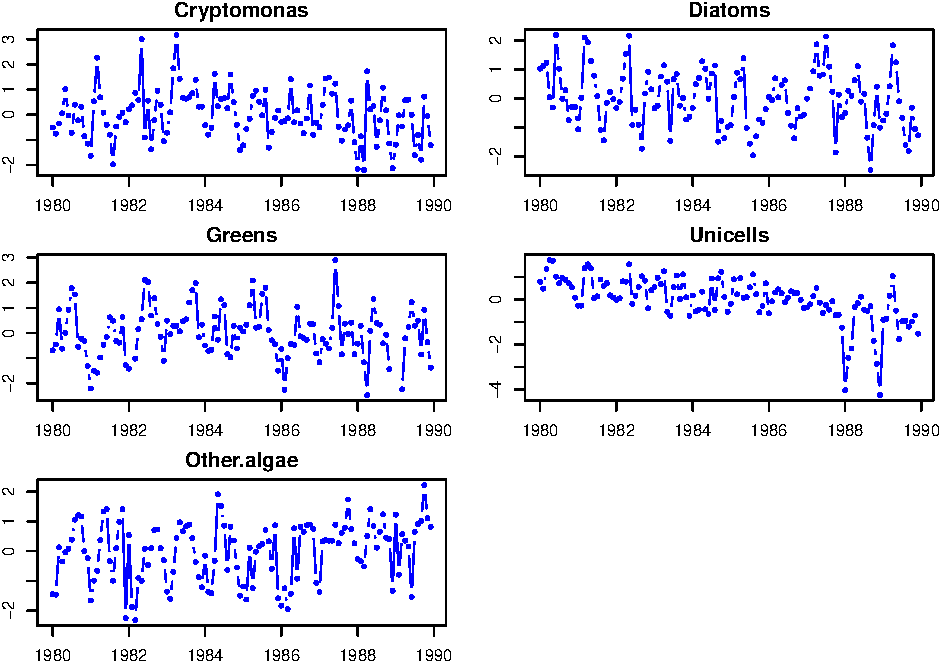
\includegraphics[width=0.8\linewidth]{fitting-models-with-stan_files/figure-latex/stan-plot-dfa-1} 

}

\caption{Phytoplankton data.}\label{fig:stan-plot-dfa}
\end{figure}

Run a 3 trend model on these data.

\begin{Shaded}
\begin{Highlighting}[]
\NormalTok{mod_}\DecValTok{3}\NormalTok{ <-}\StringTok{ }\NormalTok{bayesdfa}\OperatorTok{::}\KeywordTok{fit_dfa}\NormalTok{(}\DataTypeTok{y =}\NormalTok{ dat.spp}\FloatTok{.1980}\NormalTok{, }\DataTypeTok{num_trends =} \DecValTok{3}\NormalTok{, }
    \DataTypeTok{chains =} \DecValTok{1}\NormalTok{, }\DataTypeTok{iter =} \DecValTok{1000}\NormalTok{)}
\end{Highlighting}
\end{Shaded}

Rotate the estimated trends and look at what it produces.

\begin{Shaded}
\begin{Highlighting}[]
\NormalTok{rot <-}\StringTok{ }\NormalTok{bayesdfa}\OperatorTok{::}\KeywordTok{rotate_trends}\NormalTok{(mod_}\DecValTok{3}\NormalTok{)}
\KeywordTok{names}\NormalTok{(rot)}
\end{Highlighting}
\end{Shaded}

\begin{verbatim}
[1] "Z_rot"         "trends"        "Z_rot_mean"    "Z_rot_median" 
[5] "trends_mean"   "trends_median" "trends_lower"  "trends_upper" 
\end{verbatim}

Plot the estimate of the trends.

\begin{Shaded}
\begin{Highlighting}[]
\KeywordTok{matplot}\NormalTok{(}\KeywordTok{t}\NormalTok{(rot}\OperatorTok{$}\NormalTok{trends_mean), }\DataTypeTok{type =} \StringTok{"l"}\NormalTok{, }\DataTypeTok{lwd =} \DecValTok{2}\NormalTok{, }\DataTypeTok{ylab =} \StringTok{"mean trend"}\NormalTok{)}
\end{Highlighting}
\end{Shaded}

\begin{figure}

{\centering 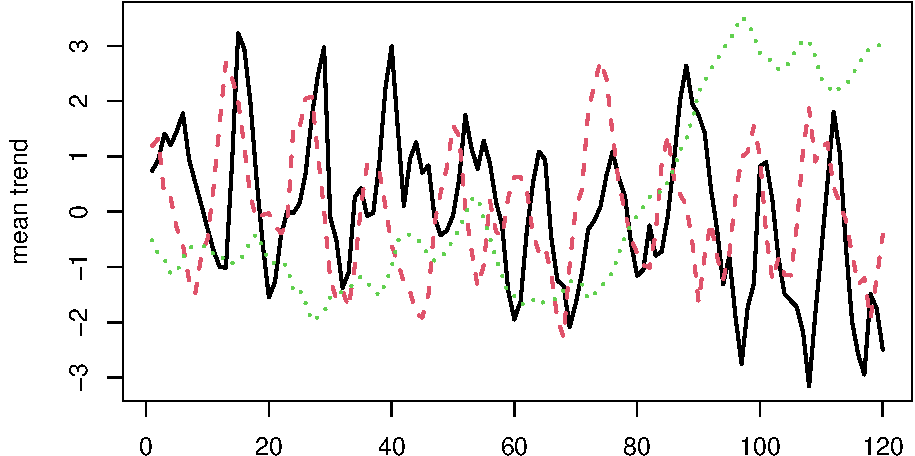
\includegraphics[width=0.8\linewidth]{fitting-models-with-stan_files/figure-latex/stan-dfa-plot-trends-1} 

}

\caption{Trends.}\label{fig:stan-dfa-plot-trends}
\end{figure}

\hypertarget{sec-stan-loo}{%
\subsubsection{Using leave one out cross-validation to select
models}\label{sec-stan-loo}}

We will fit multiple DFA with different numbers of trends and use leave
one out (LOO) cross-validation to choose the best model.

\begin{Shaded}
\begin{Highlighting}[]
\NormalTok{mod_}\DecValTok{1}\NormalTok{ =}\StringTok{ }\NormalTok{bayesdfa}\OperatorTok{::}\KeywordTok{fit_dfa}\NormalTok{(}\DataTypeTok{y =}\NormalTok{ dat.spp}\FloatTok{.1980}\NormalTok{, }\DataTypeTok{num_trends =} \DecValTok{1}\NormalTok{, }\DataTypeTok{iter =} \DecValTok{1000}\NormalTok{, }
    \DataTypeTok{chains =} \DecValTok{1}\NormalTok{)}
\NormalTok{mod_}\DecValTok{2}\NormalTok{ =}\StringTok{ }\NormalTok{bayesdfa}\OperatorTok{::}\KeywordTok{fit_dfa}\NormalTok{(}\DataTypeTok{y =}\NormalTok{ dat.spp}\FloatTok{.1980}\NormalTok{, }\DataTypeTok{num_trends =} \DecValTok{2}\NormalTok{, }\DataTypeTok{iter =} \DecValTok{1000}\NormalTok{, }
    \DataTypeTok{chains =} \DecValTok{1}\NormalTok{)}
\NormalTok{mod_}\DecValTok{3}\NormalTok{ =}\StringTok{ }\NormalTok{bayesdfa}\OperatorTok{::}\KeywordTok{fit_dfa}\NormalTok{(}\DataTypeTok{y =}\NormalTok{ dat.spp}\FloatTok{.1980}\NormalTok{, }\DataTypeTok{num_trends =} \DecValTok{3}\NormalTok{, }\DataTypeTok{iter =} \DecValTok{1000}\NormalTok{, }
    \DataTypeTok{chains =} \DecValTok{1}\NormalTok{)}
\end{Highlighting}
\end{Shaded}

\begin{verbatim}
Warning: The largest R-hat is NA, indicating chains have not mixed.
Running the chains for more iterations may help. See
http://mc-stan.org/misc/warnings.html#r-hat
\end{verbatim}

\begin{verbatim}
Warning: Bulk Effective Samples Size (ESS) is too low, indicating posterior means and medians may be unreliable.
Running the chains for more iterations may help. See
http://mc-stan.org/misc/warnings.html#bulk-ess
\end{verbatim}

\begin{Shaded}
\begin{Highlighting}[]
\NormalTok{mod_}\DecValTok{4}\NormalTok{ =}\StringTok{ }\NormalTok{bayesdfa}\OperatorTok{::}\KeywordTok{fit_dfa}\NormalTok{(}\DataTypeTok{y =}\NormalTok{ dat.spp}\FloatTok{.1980}\NormalTok{, }\DataTypeTok{num_trends =} \DecValTok{4}\NormalTok{, }\DataTypeTok{iter =} \DecValTok{1000}\NormalTok{, }
    \DataTypeTok{chains =} \DecValTok{1}\NormalTok{)}
\end{Highlighting}
\end{Shaded}

\begin{verbatim}
Warning: Bulk Effective Samples Size (ESS) is too low, indicating posterior means and medians may be unreliable.
Running the chains for more iterations may help. See
http://mc-stan.org/misc/warnings.html#bulk-ess
\end{verbatim}

\begin{Shaded}
\begin{Highlighting}[]
\CommentTok{# mod_5 = bayesdfa::fit_dfa(y = dat.spp.1980, num_trends=5)}
\end{Highlighting}
\end{Shaded}

We will compute the Leave One Out Information Criterion (LOOIC) using
the \textbf{loo} package. Like AIC, lower is better.

\begin{Shaded}
\begin{Highlighting}[]
\KeywordTok{loo}\NormalTok{(mod_}\DecValTok{1}\NormalTok{)}\OperatorTok{$}\NormalTok{estimates[}\StringTok{"looic"}\NormalTok{, }\StringTok{"Estimate"}\NormalTok{]}
\end{Highlighting}
\end{Shaded}

\begin{verbatim}
[1] 1616.017
\end{verbatim}

Table of the LOOIC values:

\begin{Shaded}
\begin{Highlighting}[]
\NormalTok{looics =}\StringTok{ }\KeywordTok{c}\NormalTok{(}
  \KeywordTok{loo}\NormalTok{(mod_}\DecValTok{1}\NormalTok{)}\OperatorTok{$}\NormalTok{estimates[}\StringTok{"looic"}\NormalTok{,}\StringTok{"Estimate"}\NormalTok{],}
  \KeywordTok{loo}\NormalTok{(mod_}\DecValTok{2}\NormalTok{)}\OperatorTok{$}\NormalTok{estimates[}\StringTok{"looic"}\NormalTok{,}\StringTok{"Estimate"}\NormalTok{],}
  \KeywordTok{loo}\NormalTok{(mod_}\DecValTok{3}\NormalTok{)}\OperatorTok{$}\NormalTok{estimates[}\StringTok{"looic"}\NormalTok{,}\StringTok{"Estimate"}\NormalTok{],}
  \KeywordTok{loo}\NormalTok{(mod_}\DecValTok{4}\NormalTok{)}\OperatorTok{$}\NormalTok{estimates[}\StringTok{"looic"}\NormalTok{,}\StringTok{"Estimate"}\NormalTok{]}
  \CommentTok{#loo::loo(loo::extract_log_lik(mod_5))$estimates["looic","Estimate"]}
\NormalTok{  )}
\NormalTok{looic.table <-}\StringTok{ }\KeywordTok{data.frame}\NormalTok{(}\DataTypeTok{trends=}\DecValTok{1}\OperatorTok{:}\DecValTok{4}\NormalTok{, }\DataTypeTok{LOOIC=}\NormalTok{looics)}
\NormalTok{looic.table}
\end{Highlighting}
\end{Shaded}

\begin{verbatim}
  trends    LOOIC
1      1 1616.017
2      2 1541.513
3      3 1475.559
4      4 1458.972
\end{verbatim}

\hypertarget{sec-stan-state-uncertainty}{%
\subsection{Uncertainty intervals on
states}\label{sec-stan-state-uncertainty}}

We will look at the effect of missing data on the uncertainty intervals
on estimates states using a DFA on the harbor seal dataset.

\begin{Shaded}
\begin{Highlighting}[]
\KeywordTok{data}\NormalTok{(harborSealWA, }\DataTypeTok{package =} \StringTok{"MARSS"}\NormalTok{)}
\CommentTok{# the first column is year}
\KeywordTok{matplot}\NormalTok{(harborSealWA[, }\DecValTok{1}\NormalTok{], harborSealWA[, }\DecValTok{-1}\NormalTok{], }\DataTypeTok{type =} \StringTok{"l"}\NormalTok{, }\DataTypeTok{ylab =} \StringTok{"Log abundance"}\NormalTok{, }
    \DataTypeTok{xlab =} \StringTok{""}\NormalTok{)}
\end{Highlighting}
\end{Shaded}

\begin{center}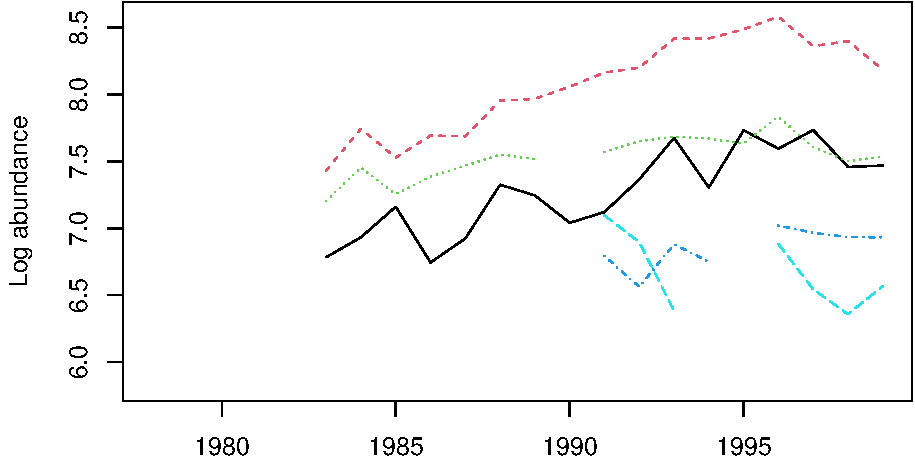
\includegraphics[width=0.8\linewidth]{fitting-models-with-stan_files/figure-latex/stan-harborseal-data-1} \end{center}

Assume they are all observing a single trend.

\begin{Shaded}
\begin{Highlighting}[]
\NormalTok{seal.mod <-}\StringTok{ }\NormalTok{bayesdfa}\OperatorTok{::}\KeywordTok{fit_dfa}\NormalTok{(}\DataTypeTok{y =} \KeywordTok{t}\NormalTok{(harborSealWA[, }\DecValTok{-1}\NormalTok{]), }\DataTypeTok{num_trends =} \DecValTok{1}\NormalTok{, }
    \DataTypeTok{chains =} \DecValTok{1}\NormalTok{, }\DataTypeTok{iter =} \DecValTok{1000}\NormalTok{)}
\end{Highlighting}
\end{Shaded}

\begin{Shaded}
\begin{Highlighting}[]
\NormalTok{pars <-}\StringTok{ }\NormalTok{rstan}\OperatorTok{::}\KeywordTok{extract}\NormalTok{(seal.mod}\OperatorTok{$}\NormalTok{model)}
\end{Highlighting}
\end{Shaded}

\begin{Shaded}
\begin{Highlighting}[]
\NormalTok{pred_mean <-}\StringTok{ }\KeywordTok{c}\NormalTok{(}\KeywordTok{apply}\NormalTok{(pars}\OperatorTok{$}\NormalTok{x, }\KeywordTok{c}\NormalTok{(}\DecValTok{2}\NormalTok{, }\DecValTok{3}\NormalTok{), mean))}
\NormalTok{pred_lo <-}\StringTok{ }\KeywordTok{c}\NormalTok{(}\KeywordTok{apply}\NormalTok{(pars}\OperatorTok{$}\NormalTok{x, }\KeywordTok{c}\NormalTok{(}\DecValTok{2}\NormalTok{, }\DecValTok{3}\NormalTok{), quantile, }\FloatTok{0.025}\NormalTok{))}
\NormalTok{pred_hi <-}\StringTok{ }\KeywordTok{c}\NormalTok{(}\KeywordTok{apply}\NormalTok{(pars}\OperatorTok{$}\NormalTok{x, }\KeywordTok{c}\NormalTok{(}\DecValTok{2}\NormalTok{, }\DecValTok{3}\NormalTok{), quantile, }\FloatTok{0.975}\NormalTok{))}

\KeywordTok{plot}\NormalTok{(pred_mean, }\DataTypeTok{type =} \StringTok{"l"}\NormalTok{, }\DataTypeTok{lwd =} \DecValTok{3}\NormalTok{, }\DataTypeTok{ylim =} \KeywordTok{range}\NormalTok{(}\KeywordTok{c}\NormalTok{(pred_mean, }
\NormalTok{    pred_lo, pred_hi)), }\DataTypeTok{main =} \StringTok{"Trend"}\NormalTok{)}
\KeywordTok{lines}\NormalTok{(pred_lo)}
\KeywordTok{lines}\NormalTok{(pred_hi)}
\end{Highlighting}
\end{Shaded}

\begin{figure}

{\centering 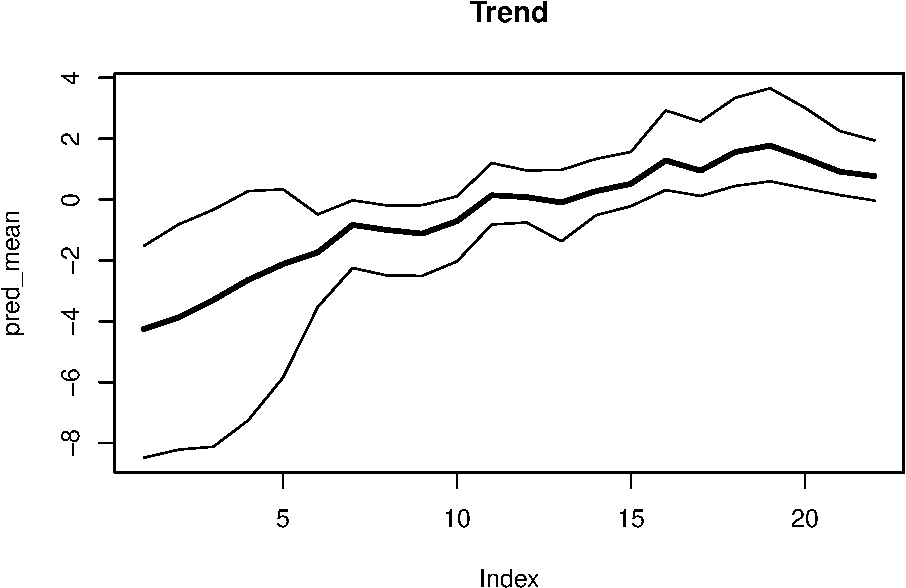
\includegraphics[width=0.8\linewidth]{fitting-models-with-stan_files/figure-latex/stan-plot-seal-1} 

}

\caption{Estimated states and 95 percent credible intervals.}\label{fig:stan-plot-seal}
\end{figure}

\hypertarget{sec-neon-data}{%
\subsection{NEON EFI Aquatics Challenge}\label{sec-neon-data}}

The data for the aquatics challenge comes from a NEON site at Lake Barco
(Florida). More about the data and challenge is
\href{https://ecoforecast.org/efi-rcn-forecast-challenges/}{here} and
the Github repository for getting all the necessary data is
\href{https://github.com/eco4cast/neon4cast-aquatics}{here}.

We can pull in the data with the code from the challenge

\begin{Shaded}
\begin{Highlighting}[]
\KeywordTok{library}\NormalTok{(tidyverse)}
\end{Highlighting}
\end{Shaded}

\begin{verbatim}
-- Attaching packages --------------------------------------- tidyverse 1.3.0 --
\end{verbatim}

\begin{verbatim}
v tibble  3.0.6     v dplyr   1.0.4
v tidyr   1.1.2     v stringr 1.4.0
v readr   1.4.0     v forcats 0.5.0
v purrr   0.3.4     
\end{verbatim}

\begin{verbatim}
-- Conflicts ------------------------------------------ tidyverse_conflicts() --
x tidyr::extract() masks rstan::extract()
x dplyr::filter()  masks stats::filter()
x dplyr::lag()     masks stats::lag()
\end{verbatim}

\begin{Shaded}
\begin{Highlighting}[]
\KeywordTok{library}\NormalTok{(lubridate)}
\end{Highlighting}
\end{Shaded}

\begin{verbatim}

Attaching package: 'lubridate'
\end{verbatim}

\begin{verbatim}
The following objects are masked from 'package:base':

    date, intersect, setdiff, union
\end{verbatim}

\begin{Shaded}
\begin{Highlighting}[]
\KeywordTok{library}\NormalTok{(rstan)}
\KeywordTok{library}\NormalTok{(ggplot2)}
\CommentTok{# This taken from code on NEON aquatics challenge}
\NormalTok{targets <-}\StringTok{ }\KeywordTok{read_csv}\NormalTok{(}\StringTok{"aquatics-targets.csv.gz"}\NormalTok{, }\DataTypeTok{guess_max =} \DecValTok{10000}\NormalTok{)}
\end{Highlighting}
\end{Shaded}

\begin{verbatim}

-- Column specification --------------------------------------------------------
cols(
  time = col_date(format = ""),
  siteID = col_character(),
  oxygen = col_double(),
  temperature = col_double(),
  oxygen_sd = col_double(),
  temperature_sd = col_double(),
  depth_oxygen = col_double(),
  depth_temperature = col_double(),
  neon_product_ids = col_character()
)
\end{verbatim}

\begin{Shaded}
\begin{Highlighting}[]
\NormalTok{site_data_var <-}\StringTok{ }\NormalTok{targets }\OperatorTok\StringTok{ }\KeywordTok{filter}\NormalTok{(siteID }\OperatorTok{==}\StringTok{ "BARC"}\NormalTok{)}

\CommentTok{# This is key here - I added the forecast horizon on the end}
\CommentTok{# of the data for the forecast period}
\NormalTok{full_time <-}\StringTok{ }\KeywordTok{tibble}\NormalTok{(}\DataTypeTok{time =} \KeywordTok{seq}\NormalTok{(}\KeywordTok{min}\NormalTok{(site_data_var}\OperatorTok{$}\NormalTok{time), }\KeywordTok{max}\NormalTok{(site_data_var}\OperatorTok{$}\NormalTok{time), }
    \DataTypeTok{by =} \StringTok{"1 day"}\NormalTok{))}

\CommentTok{# Join the full time with the site_data_var so there aren't}
\CommentTok{# gaps in the time column}
\NormalTok{site_data_var <-}\StringTok{ }\KeywordTok{left_join}\NormalTok{(full_time, site_data_var) }\OperatorTok\StringTok{ }\NormalTok{dplyr}\OperatorTok{::}\KeywordTok{rename}\NormalTok{(}\DataTypeTok{date =}\NormalTok{ time)}
\end{Highlighting}
\end{Shaded}

\begin{verbatim}
Joining, by = "time"
\end{verbatim}

\begin{Shaded}
\begin{Highlighting}[]
\NormalTok{site_data_var}\OperatorTok{$}\NormalTok{year =}\StringTok{ }\KeywordTok{year}\NormalTok{(site_data_var}\OperatorTok{$}\NormalTok{date)}
\NormalTok{site_data_var}\OperatorTok{$}\NormalTok{cal_day =}\StringTok{ }\KeywordTok{yday}\NormalTok{(site_data_var}\OperatorTok{$}\NormalTok{date)}

\KeywordTok{saveRDS}\NormalTok{(site_data_var, }\StringTok{"neon_barc.rds"}\NormalTok{)}
\end{Highlighting}
\end{Shaded}

Familiarize yourself with the oxygen and temperature data from Lake
Barco

Question: what sort of models do you think would be good candidates for
forecasting?

\hypertarget{sec-neon-oxygen}{%
\subsection{NEON EFI Aquatics Challenge}\label{sec-neon-oxygen}}

Before modeling temperature and oxygen jointly, we'll start working with
just the oxygen data alone.

We'll just with just a AR(p) state space model. The Lake Barco data has
associated standard errors with the oxygen data, so we'll use that as a
known observation error (rather than estimating that variance parameter,
in our previous work).

A script that describes the model is called \texttt{model\_01.stan}.
This should be familiar, following from the \texttt{atsar} code with a
couple modifications. First, Stan doesn't like NAs being passed in as
data, and we've had to do some indexing to avoid that. Second, notice
that the model is flexible and can be used to fit models with any
numbers of lags.

To get the data prepped for Stan, we need to do a few things. First,
specify the lag and forecast horizon

\begin{Shaded}
\begin{Highlighting}[]
\CommentTok{# Now data is ready for running our Stan models}
\NormalTok{data <-}\StringTok{ }\KeywordTok{readRDS}\NormalTok{(}\StringTok{"neon_barc.rds"}\NormalTok{)}
\NormalTok{data}\OperatorTok{$}\NormalTok{indx =}\StringTok{ }\KeywordTok{seq}\NormalTok{(}\DecValTok{1}\NormalTok{, }\KeywordTok{nrow}\NormalTok{(data))}
\NormalTok{n_forecast <-}\StringTok{ }\DecValTok{7}
\NormalTok{n_lag <-}\StringTok{ }\DecValTok{1}
\end{Highlighting}
\end{Shaded}

Next, we'll drop observations with missing oxygen. If you wanted to do
some validation, we could also split the data into a training and test
set.

\begin{Shaded}
\begin{Highlighting}[]
\CommentTok{# As a first model, we'll just work with modeling oxygen}
\NormalTok{o2_dat <-}\StringTok{ }\NormalTok{dplyr}\OperatorTok{::}\KeywordTok{filter}\NormalTok{(data, }\OperatorTok{!}\KeywordTok{is.na}\NormalTok{(oxygen))}

\CommentTok{# split the test and training data}
\NormalTok{last_obs <-}\StringTok{ }\KeywordTok{max}\NormalTok{(data}\OperatorTok{$}\NormalTok{indx) }\OperatorTok{-}\StringTok{ }\NormalTok{n_forecast}
\NormalTok{o2_train <-}\StringTok{ }\NormalTok{dplyr}\OperatorTok{::}\KeywordTok{filter}\NormalTok{(o2_dat, indx }\OperatorTok{<=}\StringTok{ }\NormalTok{last_obs)}
\NormalTok{test =}\StringTok{ }\NormalTok{dplyr}\OperatorTok{::}\KeywordTok{filter}\NormalTok{(data, indx }\OperatorTok{>}\StringTok{ }\NormalTok{last_obs)}

\NormalTok{o2_x =}\StringTok{ }\NormalTok{o2_train}\OperatorTok{$}\NormalTok{indx}
\NormalTok{o2_y =}\StringTok{ }\NormalTok{o2_train}\OperatorTok{$}\NormalTok{oxygen}
\NormalTok{o2_sd =}\StringTok{ }\NormalTok{o2_train}\OperatorTok{$}\NormalTok{oxygen_sd}
\NormalTok{n_o2 =}\StringTok{ }\KeywordTok{nrow}\NormalTok{(o2_train)}
\end{Highlighting}
\end{Shaded}

Remember that the Stan data needs to be in a list,

\begin{Shaded}
\begin{Highlighting}[]
\NormalTok{stan_data =}\StringTok{ }\KeywordTok{list}\NormalTok{(}\DataTypeTok{n =}\NormalTok{ last_obs, }\DataTypeTok{n_o2 =}\NormalTok{ n_o2, }\DataTypeTok{n_lag =}\NormalTok{ n_lag, }\DataTypeTok{n_forecast =}\NormalTok{ n_forecast, }
    \DataTypeTok{o2_x =}\NormalTok{ o2_x, }\DataTypeTok{o2_y =}\NormalTok{ o2_y, }\DataTypeTok{o2_sd =}\NormalTok{ o2_sd)}
\end{Highlighting}
\end{Shaded}

Finally we can compile the model. If we wanted to do fully Bayesian
estimates, we could do that with

\begin{Shaded}
\begin{Highlighting}[]
\NormalTok{fit <-}\StringTok{ }\KeywordTok{stan}\NormalTok{(}\DataTypeTok{file =} \StringTok{"model_01.stan"}\NormalTok{, }\DataTypeTok{data =}\NormalTok{ stan_data)}
\end{Highlighting}
\end{Shaded}

Try fitting the Bayesian model with a short chain length (maybe 1000
iterations) and 1 MCMC chain.

But because we're interested in doing this quickly, and running the
model a bunch of times, we'll try Stan's optimizing function for MAP
estimation.

\begin{Shaded}
\begin{Highlighting}[]
\NormalTok{m <-}\StringTok{ }\KeywordTok{stan_model}\NormalTok{(}\DataTypeTok{file =} \StringTok{"model_01.stan"}\NormalTok{)}
\NormalTok{o2_model <-}\StringTok{ }\NormalTok{rstan}\OperatorTok{::}\KeywordTok{optimizing}\NormalTok{(m, }\DataTypeTok{data =}\NormalTok{ stan_data, }\DataTypeTok{hessian =} \OtherTok{TRUE}\NormalTok{)}
\end{Highlighting}
\end{Shaded}

Let's extract predictions from the fitted object,

\begin{Shaded}
\begin{Highlighting}[]
\NormalTok{data}\OperatorTok{$}\NormalTok{pred =}\StringTok{ }\NormalTok{o2_model}\OperatorTok{$}\NormalTok{par[}\KeywordTok{grep}\NormalTok{(}\StringTok{"pred"}\NormalTok{, }\KeywordTok{names}\NormalTok{(o2_model}\OperatorTok{$}\NormalTok{par))]}
\KeywordTok{ggplot}\NormalTok{(data, }\KeywordTok{aes}\NormalTok{(date, pred)) }\OperatorTok{+}\StringTok{ }\KeywordTok{geom_line}\NormalTok{() }\OperatorTok{+}\StringTok{ }\KeywordTok{geom_point}\NormalTok{(}\KeywordTok{aes}\NormalTok{(date, }
\NormalTok{    oxygen), }\DataTypeTok{col =} \StringTok{"red"}\NormalTok{, }\DataTypeTok{alpha =} \FloatTok{0.5}\NormalTok{)}
\end{Highlighting}
\end{Shaded}

Question how do we evaluate predictions? We'll talk about that more next
week, but for today we can think about it as
RMSE(observations,predictions)

Question: modify the code above (just on the R side, not Stan) to fit a
lag-2 or lag-3 model. Are the predictions similar?

\hypertarget{sec-neon-oxygen-iterate}{%
\subsection{NEON EFI Aquatics Challenge}\label{sec-neon-oxygen-iterate}}

In generating forecasts, it's often a good idea to use multiple training
/ test sets. One question with this challenge is what's the best lag (or
order of AR model) for generating forecasts? Starting with lag-1, we can
evaluate the effects of different lags by starting at some point in the
dataset (e.g.~using 50\% of the observations), and generate and evaluate
forecasts. We then iterate, adding a day of data, generating and
evaluating forecasts, and repeating through the rest of the data. {[}An
alternative approach would be to adopt a moving window, where each
prediction would be based on the same number of historical data
points{]}.

I've generalized the code above into a function that takes the initial
Lake Barco dataset, and

\begin{Shaded}
\begin{Highlighting}[]
\NormalTok{create_stan_data =}\StringTok{ }\ControlFlowTok{function}\NormalTok{(data, last_obs, n_forecast, n_lag) \{}
\NormalTok{    o2_test <-}\StringTok{ }\NormalTok{dplyr}\OperatorTok{::}\KeywordTok{filter}\NormalTok{(data, indx }\OperatorTok\StringTok{ }\KeywordTok{seq}\NormalTok{(last_obs }\OperatorTok{+}\StringTok{ }\DecValTok{1}\NormalTok{, }
\NormalTok{        (last_obs }\OperatorTok{+}\StringTok{ }\NormalTok{n_forecast)))}
    
\NormalTok{    o2_train <-}\StringTok{ }\NormalTok{dplyr}\OperatorTok{::}\KeywordTok{filter}\NormalTok{(data, indx }\OperatorTok{<=}\StringTok{ }\NormalTok{last_obs, }\OperatorTok{!}\KeywordTok{is.na}\NormalTok{(oxygen))}
\NormalTok{    o2_x =}\StringTok{ }\NormalTok{o2_train}\OperatorTok{$}\NormalTok{indx}
\NormalTok{    o2_y =}\StringTok{ }\NormalTok{o2_train}\OperatorTok{$}\NormalTok{oxygen}
\NormalTok{    o2_sd =}\StringTok{ }\NormalTok{o2_train}\OperatorTok{$}\NormalTok{oxygen_sd}
\NormalTok{    n_o2 =}\StringTok{ }\KeywordTok{nrow}\NormalTok{(o2_train)}
    
\NormalTok{    stan_data =}\StringTok{ }\KeywordTok{list}\NormalTok{(}\DataTypeTok{n =}\NormalTok{ last_obs, }\DataTypeTok{n_o2 =}\NormalTok{ n_o2, }\DataTypeTok{n_lag =}\NormalTok{ n_lag, }
        \DataTypeTok{n_forecast =}\NormalTok{ n_forecast, }\DataTypeTok{o2_x =}\NormalTok{ o2_x, }\DataTypeTok{o2_y =}\NormalTok{ o2_y, }\DataTypeTok{o2_sd =}\NormalTok{ o2_sd)}
    
    \KeywordTok{return}\NormalTok{(}\KeywordTok{list}\NormalTok{(}\DataTypeTok{train =}\NormalTok{ o2_train, }\DataTypeTok{stan_data =}\NormalTok{ stan_data, }\DataTypeTok{test =}\NormalTok{ o2_test))}
\NormalTok{\}}
\end{Highlighting}
\end{Shaded}

Now we can try iterating over sets of data with a lag 1 model

\begin{Shaded}
\begin{Highlighting}[]
\NormalTok{n_forecast <-}\StringTok{ }\DecValTok{7}
\NormalTok{n_lag <-}\StringTok{ }\DecValTok{1}
\NormalTok{rmse <-}\StringTok{ }\OtherTok{NA}
\ControlFlowTok{for}\NormalTok{ (i }\ControlFlowTok{in} \DecValTok{500}\OperatorTok{:}\NormalTok{(}\KeywordTok{nrow}\NormalTok{(data) }\OperatorTok{-}\StringTok{ }\NormalTok{n_lag)) \{}
\NormalTok{    dat_list =}\StringTok{ }\KeywordTok{create_stan_data}\NormalTok{(data, }\DataTypeTok{last_obs =}\NormalTok{ i, }\DataTypeTok{n_forecast =}\NormalTok{ n_forecast, }
        \DataTypeTok{n_lag =}\NormalTok{ n_lag)}
    
    \CommentTok{# fit the model. opimizing can be sensitive to starting}
    \CommentTok{# values, so let's try}
\NormalTok{    best_map =}\StringTok{ }\FloatTok{-1e+100}
    \ControlFlowTok{for}\NormalTok{ (j }\ControlFlowTok{in} \DecValTok{1}\OperatorTok{:}\DecValTok{10}\NormalTok{) \{}
\NormalTok{        test_fit <-}\StringTok{ }\NormalTok{rstan}\OperatorTok{::}\KeywordTok{optimizing}\NormalTok{(m, }\DataTypeTok{data =}\NormalTok{ dat_list}\OperatorTok{$}\NormalTok{stan_data)}
        \ControlFlowTok{if}\NormalTok{ (test_fit}\OperatorTok{$}\NormalTok{value }\OperatorTok{>}\StringTok{ }\NormalTok{best_map) \{}
\NormalTok{            fit <-}\StringTok{ }\NormalTok{test_fit}
\NormalTok{            best_map <-}\StringTok{ }\NormalTok{test_fit}\OperatorTok{$}\NormalTok{value}
\NormalTok{        \}}
\NormalTok{    \}}
    \ControlFlowTok{if}\NormalTok{ (fit}\OperatorTok{$}\NormalTok{return_code }\OperatorTok{==}\StringTok{ }\DecValTok{0}\NormalTok{) \{}
        \CommentTok{# extract forecasts}
\NormalTok{        pred =}\StringTok{ }\NormalTok{fit}\OperatorTok{$}\NormalTok{par[}\KeywordTok{grep}\NormalTok{(}\StringTok{"forecast"}\NormalTok{, }\KeywordTok{names}\NormalTok{(fit}\OperatorTok{$}\NormalTok{par))]}
        
        \CommentTok{# evaluate predictions}
\NormalTok{        rmse[i] <-}\StringTok{ }\KeywordTok{sqrt}\NormalTok{(}\KeywordTok{mean}\NormalTok{((dat_list}\OperatorTok{$}\NormalTok{test}\OperatorTok{$}\NormalTok{oxygen }\OperatorTok{-}\StringTok{ }\NormalTok{pred)}\OperatorTok{^}\DecValTok{2}\NormalTok{, }
            \DataTypeTok{na.rm =}\NormalTok{ T))}
        
\NormalTok{    \}}
\NormalTok{\}}
\end{Highlighting}
\end{Shaded}

\hypertarget{sec-neon-oxygen-temp}{%
\subsection{NEON EFI Aquatics Challenge}\label{sec-neon-oxygen-temp}}

So far, these models have only included oxygen. We can easily bring in
the temperature data, which has it's own standard error associated with
it. We can set up a null model modeling temperature and oxygen
independently, with different lags allowed

First we have to modify our data function to also generate temperature
data.

\begin{Shaded}
\begin{Highlighting}[]
\NormalTok{create_stan_data =}\StringTok{ }\ControlFlowTok{function}\NormalTok{(data, last_obs, n_forecast, n_lag_o2, }
\NormalTok{    n_lag_temp) \{}
    \CommentTok{# create test data}
\NormalTok{    o2_test <-}\StringTok{ }\NormalTok{dplyr}\OperatorTok{::}\KeywordTok{filter}\NormalTok{(data, indx }\OperatorTok\StringTok{ }\KeywordTok{seq}\NormalTok{(last_obs }\OperatorTok{+}\StringTok{ }\DecValTok{1}\NormalTok{, }
\NormalTok{        (last_obs }\OperatorTok{+}\StringTok{ }\NormalTok{n_forecast)))}
\NormalTok{    temp_test <-}\StringTok{ }\NormalTok{dplyr}\OperatorTok{::}\KeywordTok{filter}\NormalTok{(data, indx }\OperatorTok\StringTok{ }\KeywordTok{seq}\NormalTok{(last_obs }\OperatorTok{+}\StringTok{ }
\StringTok{        }\DecValTok{1}\NormalTok{, (last_obs }\OperatorTok{+}\StringTok{ }\NormalTok{n_forecast)))}
    
\NormalTok{    o2_train <-}\StringTok{ }\NormalTok{dplyr}\OperatorTok{::}\KeywordTok{filter}\NormalTok{(data, indx }\OperatorTok{<=}\StringTok{ }\NormalTok{last_obs, }\OperatorTok{!}\KeywordTok{is.na}\NormalTok{(oxygen))}
\NormalTok{    o2_x =}\StringTok{ }\NormalTok{o2_train}\OperatorTok{$}\NormalTok{indx}
\NormalTok{    o2_y =}\StringTok{ }\NormalTok{o2_train}\OperatorTok{$}\NormalTok{oxygen}
\NormalTok{    o2_sd =}\StringTok{ }\NormalTok{o2_train}\OperatorTok{$}\NormalTok{oxygen_sd}
\NormalTok{    n_o2 =}\StringTok{ }\KeywordTok{nrow}\NormalTok{(o2_train)}
    
\NormalTok{    temp_train <-}\StringTok{ }\NormalTok{dplyr}\OperatorTok{::}\KeywordTok{filter}\NormalTok{(data, indx }\OperatorTok{<=}\StringTok{ }\NormalTok{last_obs, }\OperatorTok{!}\KeywordTok{is.na}\NormalTok{(temperature))}
\NormalTok{    temp_x =}\StringTok{ }\NormalTok{temp_train}\OperatorTok{$}\NormalTok{indx}
\NormalTok{    temp_y =}\StringTok{ }\NormalTok{temp_train}\OperatorTok{$}\NormalTok{temperature}
\NormalTok{    temp_sd =}\StringTok{ }\NormalTok{temp_train}\OperatorTok{$}\NormalTok{temperature_sd}
\NormalTok{    n_temp =}\StringTok{ }\KeywordTok{nrow}\NormalTok{(temp_train)}
    
\NormalTok{    stan_data =}\StringTok{ }\KeywordTok{list}\NormalTok{(}\DataTypeTok{n =}\NormalTok{ last_obs, }\DataTypeTok{n_lag_o2 =}\NormalTok{ n_lag_o2, }\DataTypeTok{n_lag_temp =}\NormalTok{ n_lag_temp, }
        \DataTypeTok{n_forecast =}\NormalTok{ n_forecast, }\DataTypeTok{n_o2 =}\NormalTok{ n_o2, }\DataTypeTok{o2_x =}\NormalTok{ o2_x, }\DataTypeTok{o2_y =}\NormalTok{ o2_y, }
        \DataTypeTok{o2_sd =}\NormalTok{ o2_sd, }\DataTypeTok{n_temp =}\NormalTok{ n_temp, }\DataTypeTok{temp_x =}\NormalTok{ temp_x, }\DataTypeTok{temp_y =}\NormalTok{ temp_y, }
        \DataTypeTok{temp_sd =}\NormalTok{ temp_sd)}
    
    \KeywordTok{return}\NormalTok{(}\KeywordTok{list}\NormalTok{(}\DataTypeTok{o2_train =}\NormalTok{ o2_train, }\DataTypeTok{temp_train =}\NormalTok{ temp_train, }
        \DataTypeTok{stan_data =}\NormalTok{ stan_data, }\DataTypeTok{o2_test =}\NormalTok{ o2_test, }\DataTypeTok{temp_test =}\NormalTok{ temp_test))}
\NormalTok{\}}
\end{Highlighting}
\end{Shaded}

\begin{Shaded}
\begin{Highlighting}[]
\NormalTok{m <-}\StringTok{ }\KeywordTok{stan_model}\NormalTok{(}\DataTypeTok{file =} \StringTok{"model_02.stan"}\NormalTok{)}
\end{Highlighting}
\end{Shaded}

\begin{Shaded}
\begin{Highlighting}[]
\CommentTok{# Now we can try iterating over sets of data with a lag 1}
\CommentTok{# model}
\NormalTok{n_forecast <-}\StringTok{ }\DecValTok{7}
\NormalTok{n_lag <-}\StringTok{ }\DecValTok{1}
\NormalTok{rmse <-}\StringTok{ }\OtherTok{NA}
\ControlFlowTok{for}\NormalTok{ (i }\ControlFlowTok{in} \DecValTok{500}\OperatorTok{:}\NormalTok{(}\KeywordTok{nrow}\NormalTok{(data) }\OperatorTok{-}\StringTok{ }\NormalTok{n_lag)) \{}
\NormalTok{    dat_list =}\StringTok{ }\KeywordTok{create_stan_data}\NormalTok{(data, }\DataTypeTok{last_obs =}\NormalTok{ i, }\DataTypeTok{n_forecast =}\NormalTok{ n_forecast, }
        \DataTypeTok{n_lag_o2 =}\NormalTok{ n_lag, }\DataTypeTok{n_lag_temp =}\NormalTok{ n_lag)}
    
    \CommentTok{# fit the model. opimizing can be sensitive to starting}
    \CommentTok{# values, so let's try}
\NormalTok{    best_map =}\StringTok{ }\FloatTok{-1e+100}
    \ControlFlowTok{for}\NormalTok{ (j }\ControlFlowTok{in} \DecValTok{1}\OperatorTok{:}\DecValTok{10}\NormalTok{) \{}
\NormalTok{        test_fit <-}\StringTok{ }\NormalTok{rstan}\OperatorTok{::}\KeywordTok{optimizing}\NormalTok{(m, }\DataTypeTok{data =}\NormalTok{ dat_list}\OperatorTok{$}\NormalTok{stan_data)}
        \ControlFlowTok{if}\NormalTok{ (test_fit}\OperatorTok{$}\NormalTok{value }\OperatorTok{>}\StringTok{ }\NormalTok{best_map) \{}
\NormalTok{            fit <-}\StringTok{ }\NormalTok{test_fit}
\NormalTok{            best_map <-}\StringTok{ }\NormalTok{test_fit}\OperatorTok{$}\NormalTok{value}
\NormalTok{        \}}
\NormalTok{    \}}
    
    \CommentTok{# extract forecasts}
\NormalTok{    o2_pred =}\StringTok{ }\NormalTok{fit}\OperatorTok{$}\NormalTok{par[}\KeywordTok{grep}\NormalTok{(}\StringTok{"o2_forecast"}\NormalTok{, }\KeywordTok{names}\NormalTok{(fit}\OperatorTok{$}\NormalTok{par))]}
\NormalTok{    temp_pred =}\StringTok{ }\NormalTok{fit}\OperatorTok{$}\NormalTok{par[}\KeywordTok{grep}\NormalTok{(}\StringTok{"temp_forecast"}\NormalTok{, }\KeywordTok{names}\NormalTok{(fit}\OperatorTok{$}\NormalTok{par))]}
    
\NormalTok{    pred =}\StringTok{ }\KeywordTok{c}\NormalTok{(o2_pred, temp_pred)}
\NormalTok{    obs =}\StringTok{ }\KeywordTok{c}\NormalTok{(dat_list}\OperatorTok{$}\NormalTok{o2_test}\OperatorTok{$}\NormalTok{oxygen, dat_list}\OperatorTok{$}\NormalTok{temp_test}\OperatorTok{$}\NormalTok{temperature)}
    \CommentTok{# evaluate predictions}
\NormalTok{    rmse[i] <-}\StringTok{ }\KeywordTok{sqrt}\NormalTok{(}\KeywordTok{mean}\NormalTok{((obs }\OperatorTok{-}\StringTok{ }\NormalTok{pred)}\OperatorTok{^}\DecValTok{2}\NormalTok{, }\DataTypeTok{na.rm =}\NormalTok{ T))}
    \KeywordTok{print}\NormalTok{(rmse)}
\NormalTok{\}}
\end{Highlighting}
\end{Shaded}

Question: why do the future predictions of either temp or oxygen
sometimes fall to 0, and appear to do poorly?

Question: modify the script above to loop over various oxygen and
temperature lags. Using a subset of data, say observations 500:800,
which combination yields the best predictions?

\clearpage

\hypertarget{sec-stan-problems}{%
\subsection{Problems}\label{sec-stan-problems}}

\begin{enumerate}
\def\labelenumi{\arabic{enumi}.}
\item
  By adapting the code in Section @ref(sec-stan-lr), fit a regression
  model that includes the intercept and a slope, modeling the effect of
  Wind. What is the mean wind effect you estimate?
\item
  Using the results from the linear regression model fit with no burn-in
  (Section @ref(sec-stan-burn)), calculate the ACF of the \texttt{beta}
  time series using \texttt{acf()}. Would thinning more be appropriate?
  How much?
\item
  Using the fit of the random walk model to the temperature data
  (Section @ref(sec-stan-rw)), plot the predicted values (states) and
  95\% CIs.
\item
  To see the effect of this increased flexibility in estimating the
  autocorrelation, make a plot of the predictions from the AR(1) model
  (Section @ref(sec-stan-ar1) and the RW model (@ref(sec-stan-rw)).
\item
  Fit the univariate state-space model (Section @ref(sec-stan-uss)) with
  and without the autoregressive parameter \(\phi\) and compare the
  estimated process and observation error variances. Recall that AR(1)
  without the \(\phi\) parameter is a random walk.
\item
  Run the examples related to the EFI challenge. Work through the
  questions associated with each exercise
\end{enumerate}

\end{document}
